%\begin{wrapfigure}{r}{0.5\textwidth}
 % \begin{center}
  %  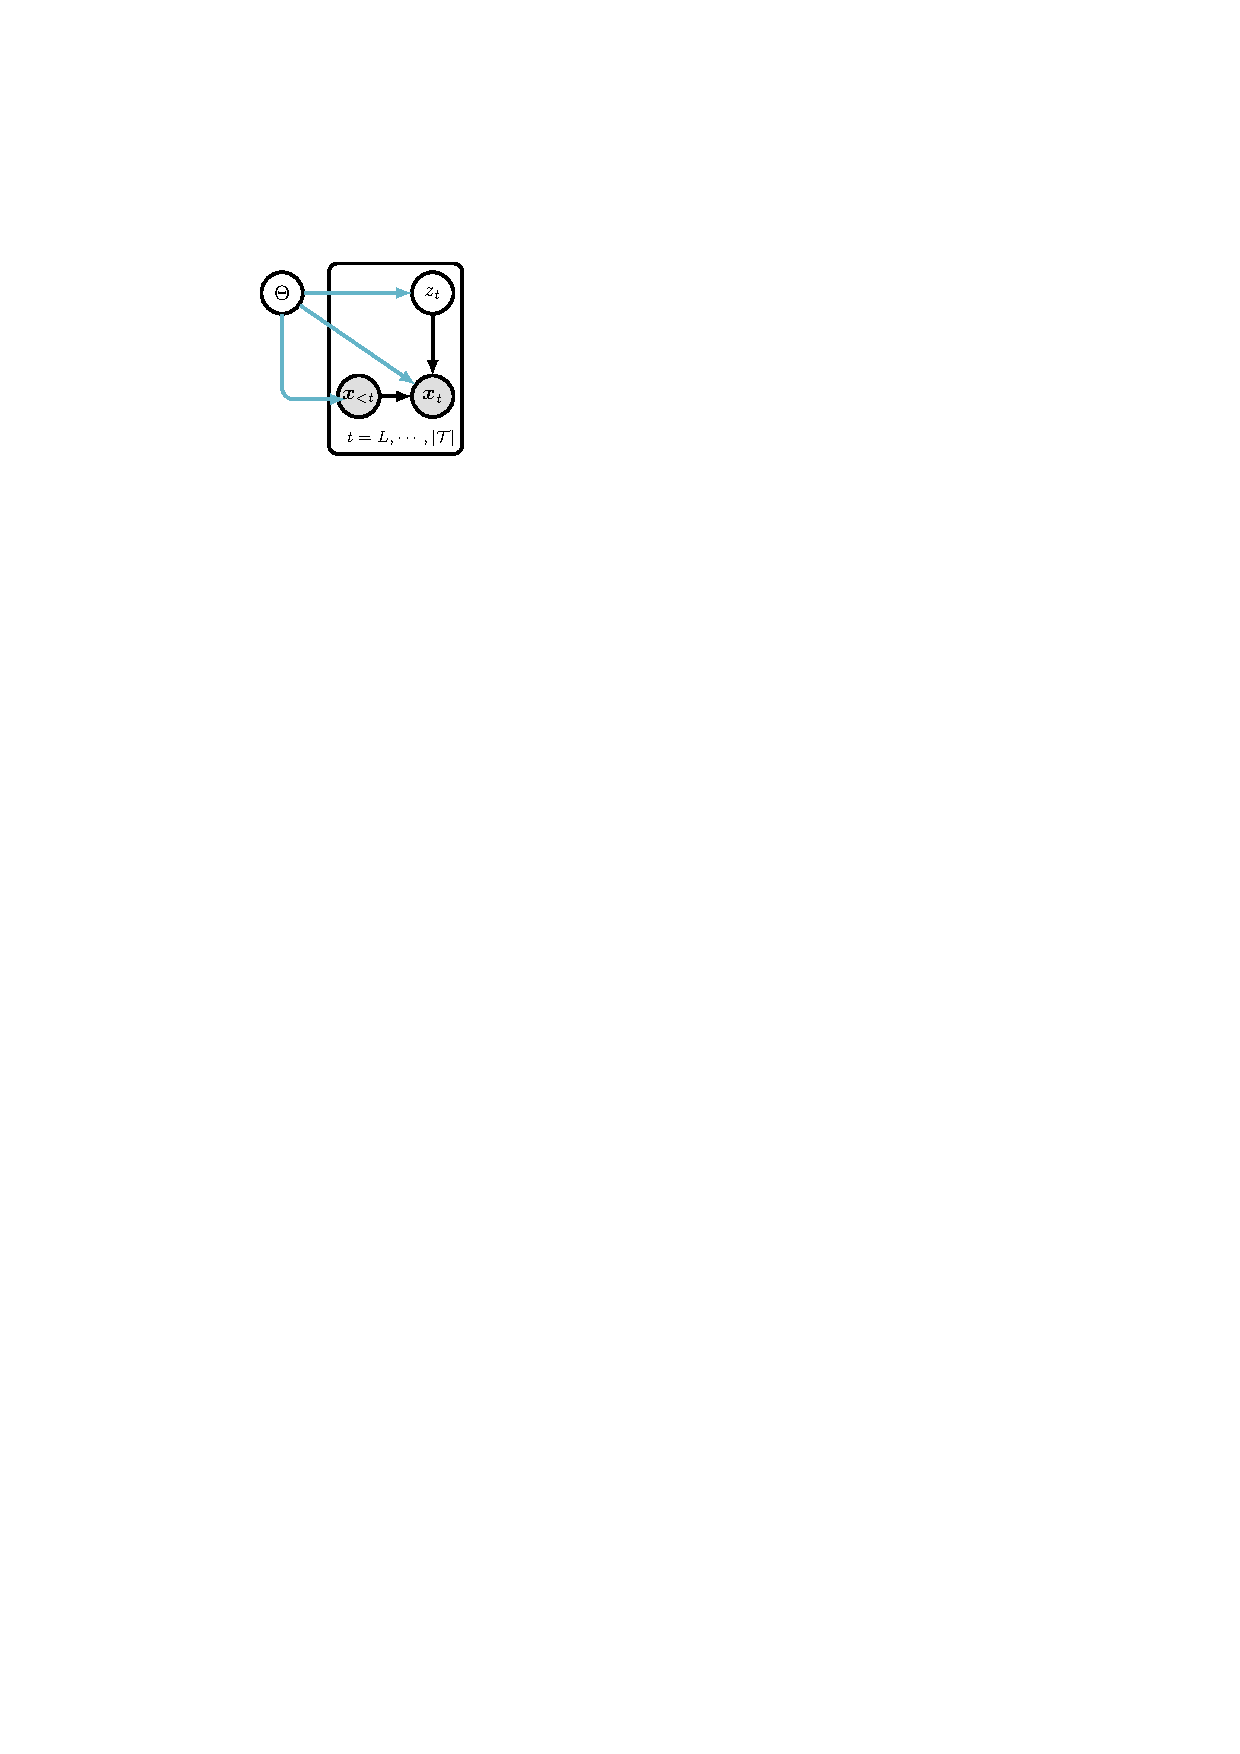
\includegraphics[width=0.25\textwidth]{figures/Fantom_graphical_model_tikz.pdf}
%\end{center}
 % \vspace{-15pt}
      %\caption{Graphical model of FANTOM. Observed variables (\(\boldsymbol{x}_t\)) are in gray, while latent variables (\(z_t\)) and parameters (\(\Theta\)) are in white. Blue edges represent parameter-variable interactions.}
     % \vspace{-45pt}
 % \label{pgm_fantom}
%\end{wrapfigure}
\section{Problem formulation}
In this Section, we introduce our notation, define a temporal causal graph, and then we present a new Structural Equation Models (SEMs) for multi-regime MTS with non-Gaussian/Heteroscedastic noise.

\textbf{Notation. } Matrices, vectors, and scalars are denoted by uppercase bold $\boldsymbol{G}_{\tau}$, lowercase bold $\boldsymbol{x}_t$ and lowercase letters $x_{t-\tau}^i$, respectively. Ground-truth variables are indicated with an asterisk, such as $\mathcal{G}^*$. We assume that all distributions have densities $p\left(\boldsymbol{x}_{t}\right)$ w.r.t. the Lebesgue measure. The notation $[|0: L|]$ represents the set of integers $\{0,...,L\}$ and $|\cdot|$ denotes set cardinality. The notation $(\boldsymbol{x}_t)_{t \in \mathcal{T}} = (x_t^i)_{i \in \mathbf{V},t \in \mathcal{T}}$ represents a MTS of $|\mathbf{V}| = d$ components and length $|\mathcal{T}|$, $\mathcal{T}$ is the time index set and $\boldsymbol{x}_{<t}$ refers to $\{\boldsymbol{x}_{t-L},...,\boldsymbol{x}_{t-1}\}$.\looseness=-1 
\begin{mybox}\begin{definition}[Temporal Causal Graph \citep{rahmanicausal}] The temporal causal graph, associated with the MTS $(\boldsymbol{x}_t)_{t \in \mathcal{T}}$, is defined by a Directed Acyclic Graph (DAG) $\mathcal{G}=(\mathbf{V}, E)$, represented by a collection of adjacency matrices $\boldsymbol{G}_{\tau \in [|0: L|]}=\{\boldsymbol{G}_{0},\dots,\boldsymbol{G}_{L}\}$, and a fixed maximum lag $L$. Its vertices $\mathbf{V}$ consist of the set of components $x_{t'}^1, \ldots, x_{t'}^d$ for each $t' \in [|t-L:t|]$. The edges $E$ of the graph are defined as follows: $\forall \tau \in [|1:L|]$ the variables $x_{t-\tau}^i$ and $x_t^j$ are connected by a lag-specific directed link $x_{t-\tau}^i \rightarrow x_t^j$ in $\mathcal{G}$ pointing forward in time if and only if $x^i$ at time $ t- \tau $ causes $x^j$ at time $t$. Then the coefficient $[G_{\tau}]_{i j}$ associated with the adjacency matrix $\boldsymbol{G}_{\tau} \in \mathcal{M}_{d}(\mathbb{R})$ will be non-zero and $x^i \in \mathbf{P a}_\mathcal{G}^j(<t)$; the lagged parents of node $i$ in $\mathcal{G}$. For instantaneous links ($\tau = 0$), we cannot have self loops i.e. $i \neq j$. If $\tau=0,\text{ we have an edge } x_{t}^i \rightarrow x_t^j \text{ and } x^i \in \mathbf{P a}_\mathcal{G}^j(t)$; the instantaneous parents of $j$ at the current time $t$, if and only if $x^i$ at time $ t$ causes $x^j$ at time $t$.
\label{definitionn1}
\end{definition}\end{mybox}
In many real world scenarios, a non-stationary MTS $(\boldsymbol{x}_t)_{t \in \mathcal{T}}$ may exhibit $K$ distinct, non-overlapping regimes, where non-stationarity is not modeled by continuous changes but rather by sequences of piecewise-constant regimes, as in climate science \citep{karmouche2023regime}, finance \citep{hamilton1994autoregressive}, or epileptic recordings \citep{wang2024ictal}.  Every regime $r$ is a stationary MTS block, has its own temporal causal graph $\mathcal{G}^r$ (Definition \ref{definitionn1}). At each time $t=1,2, \ldots, |\mathcal{T}|$ there is a discrete latent state $z_t \in\{1,2, \ldots, K\}$ that models the regime partition, i.e., $z_t = r$ means that $\boldsymbol{x}_t$ belongs to regime $r$ and we denote $\mathcal{I}_r = \{t| z_t = r, \forall t\in \mathcal{T}\}$ the set of all time indices at which regime $r$ appears. We gather these sets into $\mathcal{I} = (\mathcal{I}_r)_{r \in [|1:K|]}$, yielding a unique time partition of the MTS $(\boldsymbol{x}_t)_{t \in \mathcal{T}}$ composed of $K$ regimes. In addition, the observation $\boldsymbol{x}_t$ follows, a novel and general SEM that takes into account non stationarity, and handles both non-Gaussian case and heteroscedastic setting, that we introduce as follows, $\forall r \in [|1:K|], \forall t \in \mathcal{I}_r$:
\begin{equation}
  x_t^i= f^{i,r}\left(\mathbf{P a}_{\mathcal{G}^r}^i(<t), \mathbf{P a}_{\mathcal{G}^r}^i(t)\right)+g^{i,r}\left(\mathbf{P a}_{\mathcal{G}^r}^i(<t), \mathbf{P a}_{\mathcal{G}^r}^i(t)\right)\cdot\epsilon_t^{i,r},
\label{eq_multi_reg_hetero}
\end{equation}
where $f^{i,r}$ and $g^{i,r}$ are general differentiable functions, with $g^{i,r}$ strictly positive, and $\epsilon_t^{i,r}$ following an arbitrary probability density. We assume $\mathbb{E}(\epsilon_t^{i,r}) = 0$ and $\mathbb{E}((\epsilon_t^{i,r})^2) = 1$ without loss of generality. We denote the set of these temporal causal graphs as $\boldsymbol{\mathcal{G}} = (\mathcal{G}^r)_{r \in [|1:K|]}$. 
In the case of non-stationary MTS, regimes appear sequentially with at least a minimum duration $\zeta$, and a subsequent regime $v$ (where $v = r+1$) begins only after at least $\zeta$ time units from the start of regime $r$. Additionally, if regime $r$ reoccurs, its duration in the second appearance is also no less than $\zeta$ samples. We refer to the phenomenon, where each regime persists for at least $\zeta$ consecutive time steps, as the \emph{regime persistent dynamics} assumption and we define it as follows:
\begin{assumption}
    We consider a MTS with $K$ multiple regimes $(\boldsymbol{x}_t)_{t \in \mathcal{T}}$ where the SEM is defined in Eq.(\ref{eq_multi_reg_hetero}). Given variable $i$, we assume that a regime $r \in [|1:K|]$ is $\zeta$-persistent if the parents $(\mathbf{P a}_{\mathcal{G}^r}^i(<t), \mathbf{P a}_{\mathcal{G}^r}^i(t))$ and functional dependencies $(f^{i,r}, g^{i,r}, \epsilon_t^{i,r})$ are stationary for $\zeta$ consecutive time steps $t$.
    \label{persis_assump}
\end{assumption}
The persistence assumption permits to capture different regime dynamics, whether arising from changes in the causal graph across regimes, commonly observed in climate science \citep{karmouche2023regime} and epileptic recordings \citep{wang2024ictal}, or from shifts in functional dependencies, which correspond to soft interventions in causal discovery. Our newly introduced SEM in Eq.(\ref{eq_multi_reg_hetero}) generalizes several existing approaches in three novel aspects: (1) when $K=1$, if $g^{i,1}(\mathbf{Pa}_{\mathcal{G}^1}^i(<t), \mathbf{Pa}_{\mathcal{G}^1}^i(t)) = 1$ for all $i \in [|1:d|]$, we recover the classical additive noise models in causal discovery. Thus, allowing $g^{i,1}$ to be a strictly positive and differentiable function,  \textit{not only extends Rhino’s SEM \citep{gong2022rhino} but also yields a new, general SEM for stationary multivariate time series with heteroscedastic noise}.  (2) When $K>1$, if $g^{i,1}(\mathbf{Pa}_{\mathcal{G}^r}^i(<t), \mathbf{Pa}_{\mathcal{G}^r}^i(t)) = 1$, and $\epsilon_t^{i,r} \sim \mathcal{N}(0, \sigma_r)$ for all $i \in [|1:d|]$, we recover the setting introduced in \citep{rahmanicausal,balsells2023identifiability}. Then, allowing $\epsilon_t^{i,r}$ to follow an arbitrary probability density then yields the first \textit{SEM for non-stationary MTS composed of multiple regimes with non-Gaussian noise}. Finally, (3) permitting $g^{i,r}$ to be a strictly positive, differentiable function leads, to the best of our knowledge, to the first \textit{general SEM for non-stationary MTS with heteroscedastic noise}.\looseness=-1

